% For tips on writing the thesis, see http://www.tug.org/pracjourn/2008-1/mori/mori.pdf

% Two side to save paper
% openrigth means to put the chapter tittle on the right pages
\documentclass[12pt,letterpaper,twoside,openright]{book}
\usepackage[utf8x]{inputenc}
\usepackage[T1]{fontenc}
% Language support
\usepackage[english,spanish]{babel}

\usepackage[table,xcdraw]{xcolor}


\newenvironment{dedication}
{
   \cleardoublepage
   \thispagestyle{empty}
   \vspace*{\stretch{1}}
   \hfill\begin{minipage}[t]{0.66\textwidth}
   \raggedright
}%
{
   \end{minipage}
   \vspace*{\stretch{3}}
   \clearpage
}

\newenvironment{acreditation}
{
   \cleardoublepage
   \thispagestyle{empty}
   %\vspace*{\stretch{1}}
   
   %\raggedright
}%
{
   
   %\vspace*{\stretch{3}}
   \clearpage
}


\newenvironment{notetoeditor}
{
   \begin{tcolorbox}[title={Nota al editor},colback=yellow!5!white]
}%
{
   \end{tcolorbox}
}

\newcommand*{\captionsource}[2]{%
	\caption[{#1}]{%
		#1%
		\\\hspace{\linewidth}%
		\textbf{Source:} #2%
	}%
}

\setcounter{tocdepth}{4}
\setcounter{secnumdepth}{4}

\selectlanguage{english}
%\usepackage[spanish]{datetime}

% We define some strings that will use along
\def \thesiskeywords {thesis, master degree, your topics here}
\def \pdfauthor {Student Name Here}
\def \thesistitle{Thesis Title Goes Here}

% Custom-commands and definitions
% See this file for defining the keywords that will show up on the PDF file
%For spanish we need indentation on the first line
%\usepackage{indentfirst}

%math package
\usepackage{amsthm}
\usepackage{amsmath}
\usepackage{amssymb}
\usepackage{pseudocode}

\newcommand{\lstnumberautorefname}{Listing}


\newtheorem{definition}{Definition}[subsection]
\newcommand{\definitionautorefname}{Definition}

\newtheorem{theorem}{Theorem}[subsection]
\newtheoremstyle{theorem}{}{}{\itshape}{}{\bfseries}{.}{.5em}{\thmnote{#3's }#1}
\newcommand{\theoremautorefname}{Theorem}

\newtheorem{lemma}{Lemma}[subsection]
\newtheoremstyle{lemma}{}{}{\itshape}{}{\bfseries}{.}{.5em}{\thmnote{#3's }#1}
\newcommand{\lemmaautorefname}{Lemma}

\newtheorem*{remark}{Remark}
\newcommand{\remarkautorefname}{Remark}

\newcommand{\algorithmautorefname}{Algorithm}

\usepackage{listings}

\lstdefinestyle{customc}{
  language=C++,
  belowcaptionskip=1\baselineskip,
  breaklines=true,
  frame=l,
  xleftmargin=\parindent,
  showstringspaces=false,
  basicstyle=\linespread{0.9}\scriptsize,
  emptylines=0,
  keywordstyle=\scriptsize\ttfamily\bfseries\color{blue!40!black},
  commentstyle=\mdseries\scriptsize\color{gray!40!black},
  identifierstyle=\scriptsize\ttfamily\color{darkgray!15!black},
  stringstyle=\scriptsize\ttfamily\color{green!40!black},
}

\lstset{style=customc}

\usepackage{textcomp}
\DeclareUnicodeCharacter{8208}{fi}

\usepackage{supertabular}

%tables
\usepackage{multirow}
\usepackage{booktabs}
%\usepackage[table]{xcolor}

%figures in the exact position as code
\usepackage{float}

% Prevent latex from expanding to fill page
\raggedbottom

%Use the margins requested
\usepackage[hmargin={3.5cm,2.5cm},vmargin=2.5cm]{geometry}

%bold font for caption
\usepackage[labelfont=bf]{caption}

%\usepackage{digsig}

%Improved bibliography
\usepackage[round,sort,numbers,authoryear]{natbib}
\usepackage{usebib}
\bibpunct{[}{]}{;}{n}{,}{,}

% To define spacing
\usepackage{setspace}

% Bible references
\usepackage{verse}
\usepackage{bibleref}

% We use these packages for making the nice logo on the title page
\usepackage[pdftex]{graphicx}

%chemical
\usepackage{chemformula}

% Use input characters instead of scape codes
\usepackage[utf8x]{inputenc}

% Generate fancy chapter titles
\usepackage[Sonny]{fncychap}
\ChNameAsIs
\ChNumVar{\Large}
\ChNameVar{\fontsize{50}{60}}

%no word breaking
%\usepackage[none]{hyphenat}
\tolerance=1
\emergencystretch=\maxdimen
\hyphenpenalty=10000
\hbadness=10000

%Use Fancy headers
\usepackage{fancyhdr}
%\pagestyle{fancy}
%\fancyhead[LO]{\nouppercase{\leftmark}}
\lhead{\nouppercase{\rightmark}}

% Generate pretty PDF with links on the TOC
\usepackage{mdwlist}
\usepackage{alltt}
\usepackage[bookmarks=true,linktoc=all, colorlinks=true, pdftitle={\thesistitle}, pdfauthor={\pdfauthor}, pdfsubject={\thesistitle}, pdfkeywords={\thesiskeywords},
linkcolor=darkgray,filecolor=darkgray,urlcolor=darkgray,citecolor=darkgray]{hyperref}


\addto\extrasenglish{%
  \renewcommand{\chapterautorefname}{Chapter}%
  \renewcommand{\sectionautorefname}{Section}%
  \renewcommand{\subsectionautorefname}{Section}%
  \renewcommand{\subsubsectionautorefname}{Section}%
}

\newcommand*{\fullref}[1]{\hyperref[{#1}]{\autoref*{#1}, \nameref*{#1}}} % One single link

\newcommand*{\listingref}[1]{\hyperref[{#1}]{\autoref*{#1} \nameref*{#1} [page~\pageref{#1}]}}

% Allow epigraphs at the beginning of chapters
\usepackage{epigraph}
\setlength{\epigraphrule}{0pt}
\setlength{\afterepigraphskip}{10pt}

% Define abstract environment since it doesn't exists on book class
\newenvironment{abstract}%
{\cleardoublepage\null \vfill \begin{center}%
\bfseries \abstractname \end{center}}
{\vfill\null}

% Generation of nomenclature
\usepackage{nomencl}
\makenomenclature

% Generation of acronyms
\usepackage[footnote,withpage,printonlyused]{acronym}

% For color definitions
\usepackage{color}

% Comment this out when is not a draft
%\usepackage{draftwatermark}
%\SetWatermarkLightness{0.95}
%\SetWatermarkFontSize{5cm}
%\SetWatermarkScale{5}
%\SetWatermarkText{DRAFT}

% Custom commands
\newcommand{\HRule}{\rule{\linewidth}{0.5mm}}

\usepackage{cclicenses}

\usepackage{soulutf8}
\usepackage{varwidth}

\definecolor{light-gray}{gray}{0.75}

\newcommand\backBox[1]{%
  \colorbox{light-gray}{\begin{varwidth}{\dimexpr\linewidth-2\fboxsep}#1\end{varwidth}}}
  
\newcommand\hightligher[1]{%
  \colorbox{yellow}{\begin{varwidth}{\dimexpr\linewidth-2\fboxsep}#1\end{varwidth}}}
  
  
\usepackage{tcolorbox}
\usepackage{tabularx}
\newcolumntype{L}{>{\raggedright\arraybackslash}X}
\usepackage{array}
\usepackage{colortbl}

\newcolumntype{Y}{>{\raggedleft\arraybackslash}X}

\tcbset{tab1/.style={fonttitle=\bfseries\large,fontupper=\normalsize\sffamily,
colback=white!10!white,colframe=red!75!black,colbacktitle=white!40!white,
coltitle=black,center title,freelance,frame code={
\foreach \n in {north east,north west,south east,south west}
{\path [fill=gray!75!black] (interior.\n) circle (3mm); };},}}

\tcbset{tab2/.style={fonttitle=\bfseries,fontupper=\normalsize\sffamily,
colback=white!10!white,colframe=gray!50!black,colbacktitle=white!40!white,
coltitle=black,center title}}

\usepackage{pgfgantt}
\usepackage{soul}
%\include{eshyph.tex}
\usepackage{tikz}
\usepackage{verbatim}
\usetikzlibrary{calc,trees,positioning,arrows,chains,shapes.geometric,%
    decorations.pathreplacing,decorations.pathmorphing,shapes,%
    matrix,shapes.symbols}

\tikzset{
>=stealth',
  punktchain/.style={
    rectangle, 
    rounded corners, 
    % fill=black!10,
    draw=black, very thick,
    text width=10em, 
    minimum height=3em, 
    text centered, 
    on chain},
  line/.style={draw, thick, <-},
  element/.style={
    tape,
    top color=white,
    bottom color=blue!50!black!60!,
    minimum width=8em,
    draw=blue!40!black!90, very thick,
    text width=10em, 
    minimum height=3.5em, 
    text centered, 
    on chain},
  every join/.style={->, thick,shorten >=1pt},
  decoration={brace},
  tuborg/.style={decorate},
  tubnode/.style={midway, right=2pt},
}

\usepackage{pdflscape}
\usepackage{svg}

% TODO List support

\usepackage{xargs}                      % Use more than one optional parameter in a new commands

\usepackage{algorithm}
\usepackage[noend]{algpseudocode}


\usepackage[colorinlistoftodos,prependcaption,textsize=tiny]{todonotes}
\newcommandx{\unsure}[2][1=]{\todo[linecolor=red,backgroundcolor=red!25,bordercolor=red,#1]{#2}}
\newcommandx{\change}[2][1=]{\todo[linecolor=blue,backgroundcolor=blue!25,bordercolor=blue,#1]{#2}}
\newcommandx{\addsummary}[2][1=]{\todo[linecolor=yellow,backgroundcolor=yellow!25,bordercolor=yellow,#1]{Add summary of: #2}}

\newcommandx{\addmoreinfo}[2][1=]{\todo[linecolor=yellow,backgroundcolor=yellow!25,bordercolor=yellow,#1]{Add more information about: #2}}

\newcommandx{\rewritethis}[2][1=]{\todo[linecolor=pink,backgroundcolor=pink!25,bordercolor=pink,#1]{Rewrite: #2}}

\newcommandx{\improvement}[2][1=]{\todo[linecolor=green,backgroundcolor=green!25,bordercolor=green,#1]{#2}}
\newcommandx{\thiswillnotshow}[2][1=]{\todo[disable,#1]{#2}}


\newcommand{\presentationitem}[1]{%
\iftoggle{paper}
{
  \subsubsection{#1}
}
{
  \item
  \def\@currentlabelname{#1}%
  \textbf{#1}
}
}

\newcommand{\presentationitembig}[1]{%
\iftoggle{paper}
{
  \subsection{#1}%
}%else
{%
  \item%
  \textbf{#1:}%
  \def\@currentlabelname{\emph{#1}}%
}
}


\newenvironment{wbstaks}
{
}
{
}

\newcommand{\presentationbreak}{}

\usetikzlibrary{decorations.text,calc,arrows.meta}


\usetikzlibrary{lindenmayersystems,arrows.meta}
\newcount\quadrant
\pgfdeclarelindenmayersystem{cayley}{
  \rule{A -> B [ R [A] [+A] [-A] ]}
  \symbol{R}{ \pgflsystemstep=0.5\pgflsystemstep } 
  \symbol{-}{
    \pgfmathsetcount\quadrant{Mod(\quadrant+1,4)}
    \tikzset{rotate=90}
  }
  \symbol{+}{
    \pgfmathsetcount\quadrant{Mod(\quadrant-1,4)}
    \tikzset{rotate=-90}
  }
  \symbol{B}{
    \draw [dot-cayley] (0,0) -- (\pgflsystemstep,0) 
       node [font=\footnotesize, midway, 
         anchor={270-mod(\the\quadrant,2)*90}, inner sep=.5ex] 
           {\ifcase\quadrant$a$\or$b$\or$c$\or$d$\fi};
    \tikzset{xshift=\pgflsystemstep}
  }
}
\tikzset{
  dot/.tip={Circle[sep=-1.5pt,length=3pt]}, cayley/.tip={Stealth[]dot[]}
}

%Glossary
\usepackage[toc,acronym]{glossaries}

\usepackage{csvsimple}

% Remove this
\usepackage{todonotes}




\newtoggle{paper}
\settoggle{paper}{true}

\usepackage{csvsimple}


\begin{document}

% This is the first part of the document (frontmatter), use Roman numeration
\frontmatter

% Simple style
\pagestyle{empty}

% The front page of the thesis is in this page, Name of the school and the program can be changed here. Supervisor name gets changed here.
\selectlanguage{english}
\begin{titlepage}

\begin{center}

\vfill



\includegraphics[width=1\textwidth]{../images/TECRGB.jpg}
\\[0.2cm]
\definecolor{tecblue}{rgb}{0.016,0.173,0.322}
\textcolor{tecblue}{
\textsc{\LARGE Escuela de Ingeniería en Computación}\\[0.2cm]
\textsc{\large Programa de Maestría en Computación}\\
}
\vfill
% Title
\HRule
\\[0.9cm]
\doublespacing
{ \huge \bfseries \thesistitle}
\\[0.4cm]
\singlespacing
\HRule
\\[0.9cm]

{\large Thesis proposal submitted in partial fulfilment to opt for the degree of 
\\[1cm]
\textit{Magister Scientiæ} in Computer Science}
\\
\vfill
 
 % Author and supervisor
\begin{minipage}{0.45\textwidth}
\begin{flushleft} \large
Author\\
\pdfauthor 
\end{flushleft}
\end{minipage}
\begin{minipage}{0.50\textwidth}
\begin{flushright} \large
Supervisor\\
\pdfsupervisor
\end{flushright}
\end{minipage}
 
 
\vfill
 
% Bottom of the page
{\large \today \\}  \hfill{} 

%\cludegraphics{../imagenes/cc.png} \\
%Liberado con una licencia Creative Commons Atribución, Compartir igual.

\end{center}
\end{titlepage}

%\digsigfield{5cm}{3cm}{julatec}

%

\selectlanguage{spanish}
%\begin{acreditation}
% The ghesis act goes here.
%\makebox[\linewidth]{
    
\includegraphics[width=0.75\paperwidth,height=1\paperheight]{../images/certificate.pdf}
%}

%\end{acreditation}


\begin{dedication}
\selectlanguage{english}
If the author wants, he can put a dedication here. 
\HRule\\
\selectlanguage{spanish}
Y la versión en español puede ir acá.
\selectlanguage{english}
\end{dedication}

%%%%%%%%%ISSUE NUMBER 1%%%%%%%%%%%
\chapter*{Acknowledgements}
\doublespacing
This section can be used for the acknowledgements.

% The abstract is included on a separte file here
\newpage
\thispagestyle{empty}
\mbox{}

% Now let put the abstract in two languages
\doublespacing

\selectlanguage{english}%
\begin{abstract}
\iftoggle{paper}
{
The body of the abstract goes here.
 
}%


\end{abstract}

%\selectlanguage{spanish}%
%\begin{abstract}
%\input{body/resumen-text}
%\end{abstract}

\selectlanguage{english}


%\singlespace


%Table of contents is generated here
\tableofcontents

%List of figures goes here
\listoffigures

%List of tables is generated here
\listoftables

\mainmatter
% Use double space
\doublespacing
% Now fancy style
\pagestyle{fancy}
\setlength{\headheight}{14.5pt}
% Left the right header clean
\rhead{}

\renewcommand{\chaptername}{Chapter}

\doublespacing

% The section introduction is included
\chapter{Introduction}
\label{chapter:introduction}
%
%
%Introduction section goes here. Here is an example reference
%\cite{examplereference}. Here is another example reference \cite{examplereference2}.

Facial Expression Recognition (FER) plays a critical role in various fields such as human-computer interaction, affective computing, and security systems, where understanding human emotions through facial cues is essential. The advent of deep learning, particularly transformer-based architectures, has significantly advanced the performance of FER systems. One such promising approach is the Visual Transformer (ViT), which excels in capturing spatial relationships in image data through self-attention mechanisms.

In this context, POSTER \cite{zheng_poster_2022} stands out as an effective model for extracting multi-scale features, combining both local and global representations to improve facial expression classification. However, despite the potential of POSTER, there remains room for improvement in how it integrates learned features for final prediction. By modifying the MLP architecture, it is possible to better utilize the rich features learned by POSTER, leading to improved classification performance, especially for subtle or difficult-to-distinguish facial expressions. 


This research proposes to enhance FER models by incorporating changes to the MLP layers, focusing on dropout strategies, layer depth, and activation functions.The aim of this study is to combine the strengths of POSTER’s multi-scale feature extraction with optimizations to the MLP for more effective feature fusion and decision-making. Through this combination, the research seeks to improve the recognition of facial expressions, particularly in challenging or in-the-wild scenarios. 

\newpage

\section{Problem}

%Problem context, description and summary goes in this section:

%Multiple studies have explored the use of Visual Transformers and attention mechanisms for FER, particularly in challenging real-world conditions (e.g., occlusions, varying poses). For instance, there has been extensive work on hybrid Vision Transformers (ViTs) combined with Convolutional Neural Networks (CNNs), focusing on improving feature extraction and recognition by capturing both local and global features.
%
%However, the specific approach of modifying the MLP head architecture has not been extensively explored, making it a potentially novel contribution. Current work often focuses on the Transformer architecture itself, with enhancements like selective attention fusion. Recent investigations have not delved deeply into modifications at the classification head level.

Facial Expression Recognition (FER) is a critical area of research in computer vision with numerous applications, such as human-computer interaction, mental health monitoring, and affective computing. Despite significant advancements, FER remains a challenging task due to the inherent variability in real-world conditions, such as occlusions, varying lighting, and diverse facial poses. These challenges necessitate robust models capable of accurately capturing and interpreting subtle emotional cues across diverse scenarios.

In recent years, Visual Transformers (ViTs) have emerged as a powerful alternative to traditional Convolutional Neural Networks (CNNs) in FER tasks. Their ability to leverage self-attention mechanisms enables them to capture long-range dependencies and global contextual information, making them well-suited for FER. 

Several hybrid approaches have combined ViTs with CNNs to exploit the strengths of both architectures, aiming to enhance feature extraction by integrating both local and global features. These approaches often achieve state-of-the-art performance, particularly in controlled environments.

However, a critical limitation of existing research lies in its predominant focus on architectural innovations within the Transformer backbone or selective attention mechanisms. For example, efforts have been directed toward enhancing the encoder layers, incorporating pyramid fusion strategies, or developing cross-attention mechanisms to improve feature representation. While these advancements contribute to model performance, the exploration of modifications in the classification head particularly the Multi-Layer Perceptron (MLP) head has been relatively overlooked.

The classification head plays a essential role in transforming learned features into final predictions. Modifying the MLP head architecture offers a promising avenue for innovation, as it directly impacts the model's ability to generalize and interpret high-dimensional embedding effectively. Despite its importance, few studies have explored alternative configurations, activation functions, or dropout strategies in this component. This represents a significant opportunity for meaningful contributions to FER research.

By addressing this gap, the proposed research aims to investigate novel modifications to the MLP head in Visual Transformers for FER. This includes experimenting with advanced architectures, integrating recurrent layers and evaluating the impact of these changes on model performance under real-world conditions. Such an approach has the potential to provide deeper insights into the role of classification heads in FER, ultimately paving the way for more robust and adaptable models.



\section{Document Structure}

The document is structured into several key sections, starting with the Introduction, which presents the research topic, the problem being addressed, and an overview of the document's organization. The Theoretical Framework follows, providing background information on Facial Expression Recognition (FER), including emotional labeling, challenges in real-world scenarios, deep learning approaches, visual transformers, performance evaluation metrics, and related work. Next, the Hypothesis and Objectives section defines the research hypothesis, main and specific objectives, expected deliverables, and the scope and limitations of the study. 

The Research Proposal section outlines the proposed methodology, experiment design, variables, statistical tools, and data collection process, detailing specific elements such as response variables and the dataset used. The Preliminary Results section presents initial findings, followed by Conclusions and Future Work, summarizing the outcomes and suggesting potential future directions. Finally, the document includes Appendixes for supplementary materials and a References section citing relevant sources. This structured approach ensures clarity in the research reading and a logical progression from problem identification to experimentation and evaluation.



% Theoretical framework contents
\chapter{Theoretical Framework}
\label{chapter:theoretical-framework}


This chapter describes the theoretical concepts needed to understand the work that will be developed during the research's execution.


\section{FER}

\subsection{Emotional Labeling}

\subsection{FER in-the-wild}

\section{FER Archiquectures}

\subsection{Deep Learning for FER}

\subsection{Visual Transformer}

\section{FER Performance and Evaluation}


\subsection{Performance Metrics for FER}

\subsection{Evaluation of Modified Heads}

\cite{dosovitskiy_image_2021}

%\section{Concept 1}
%
%\label{section:Concept1}
%
%First theoretical framework concept goes here.
%
%\subsection{Subsection of Concept 1} 
%\subsection{Subsection 2 of Concept 1}
%Some text goes here \cite{examplereference}. An example of displaying and referencing an image is shown in \textbf{Figure \ref{fig:example}}
%
%
%\begin{figure}
%	\begin{center}
%		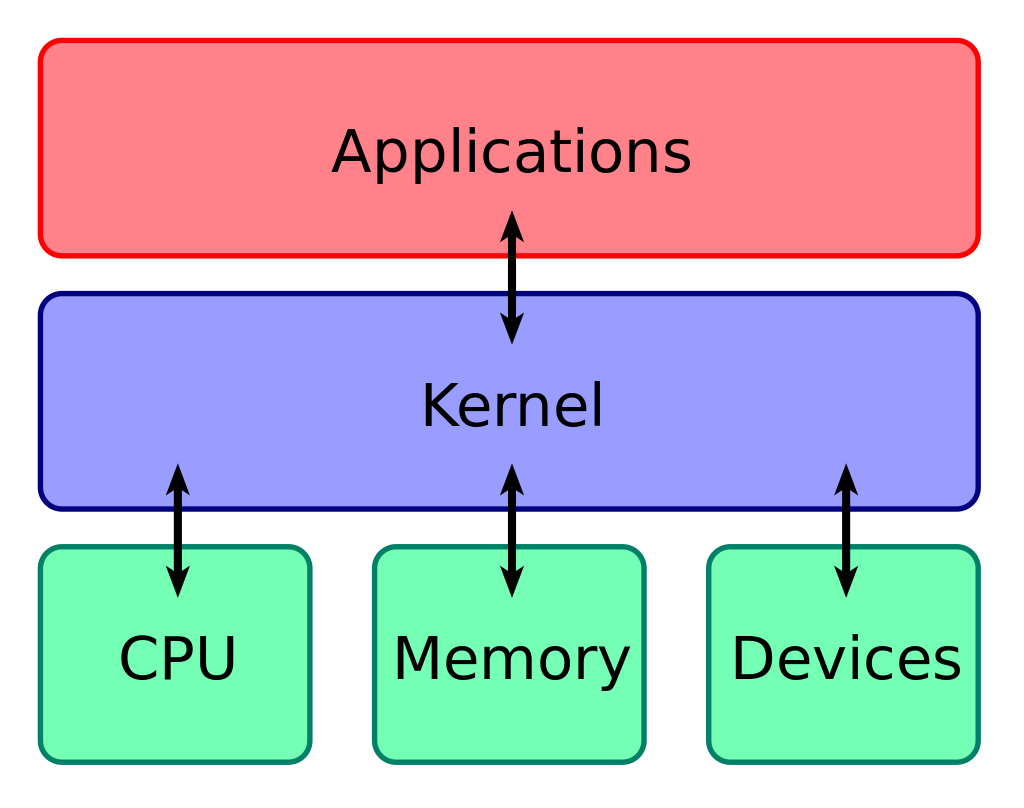
\includegraphics[width=1\columnwidth]{../img/image.png}
%		\caption[]{Example image with reference \cite{examplereference}.}
%		\label{fig:example}
%	\end{center}
%\end{figure}
%
%
%\section{Concept 2}
%
%\label{section:Concept2}
%
%\subsection{Subsection Concept 2}
%
%\subsubsection{Subsection 2 Concept 2}
%
%\section{Concept 3}
%An example of pseudo-code can be seen in \textbf{Algorithm \ref{examplepseudocode}}
%
%\begin{pseudocode}{Pseudo\_Code}{Input} \label{examplepseudocode}
%	\FOR y \GETS 1 \TO Input.MaxL \DO
%	\BEGIN
%	\FOR x \GETS 1 \TO Input.MaxH \DO
%	\BEGIN
%	a \GETS \CALL {FunctionCall}{x,y}\\
%	b \GETS \CALL {AnotherFunction}{x, y}\\
%	\CALL {ThirdFunction}{a,b}
%	\END
%	\END
%\end{pseudocode}
%
%
%\subsection{Example equation}
% Equation \ref{eq:1} shows an example equation.
%
%\[
%I=(L\cdot N) \tag{1} \label{eq:1}
%\]
  
\section{Related Work}
The related work for the research is include in this section:

Facial expression recognition (FER) has been extensively studied over the past decades, evolving from traditional machine learning approaches to deep learning methods. Early FER systems relied on handcrafted features such as Local Binary Patterns (LBP) and Histogram of Oriented Gradients (HOG). These approaches, while computationally efficient, often struggled to generalize across diverse datasets due to limited feature representation capabilities. 

The advent of convolutional neural networks (CNNs) revolutionized FER by enabling automatic feature extraction, with architectures such as VGGNet, ResNet \cite{he_deep_2015}, and EfficientNet achieving significant performance improvements. However, CNNs face limitations in capturing global dependencies and spatial relationships in images, which has motivated the exploration of transformer-based models in computer vision tasks \cite{islam_recent_2023}.

The introduction of Vision Transformers (ViTs) by Dosovitskiy \cite{dosovitskiy_image_2021} marked a significant shift in how visual tasks are approached. By leveraging self-attention mechanisms, ViTs can model long-range dependencies and capture richer contextual information compared to traditional CNNs.

Subsequent works have refined transformer architectures for visual tasks, including pyramid-based models that enhance multi-scale feature representation\cite{zheng_poster_2022}. For FER, transformer-based methods have shown promise by addressing challenges such as subtle facial expression variations and occlusions. Notably, pyramid transformers, such as those used in POSTER, offer hierarchical feature extraction capabilities that are particularly beneficial for FER.



\begin{table}[H]
\centering
\caption{State of the Art of FER systems}
\renewcommand{\arraystretch}{1.5} % Adjust row spacing
\begin{tabular}{llll}
\hline
\textbf{Model}   & \textbf{Accuracy (\%)} & \textbf{Parameters (M)} & \textbf{Key Insights}                                                                                                       \\ \hline
ResNet-50   \cite{he_deep_2015}     & 86.34                  & 24.6 & \begin{tabular}[c]{@{}l@{}}Baseline CNN with strong local \\ feature extraction but lacks \\ global context.\end{tabular}   \\
Swin Transformer \cite{lixu_swin_2021} & 90.97                & 28.3                    & \begin{tabular}[c]{@{}l@{}}Hierarchical ViT with local-global \\ features but computationally \\ expensive.\end{tabular}    \\
ViT (Base)  \cite{dosovitskiy_image_2021}     & 86.34                 & 86.4               & \begin{tabular}[c]{@{}l@{}}Standard transformer struggles \\ with subtle FER cues in \\ real-world conditions.\end{tabular} \\
\textbf{POSTER} \cite{zheng_poster_2022}  & \textbf{92.05}         & \textbf{Not specified}           & \begin{tabular}[c]{@{}l@{}}Combines pyramid attention and \\ cross-fusion for local-global \\ feature synergy.\end{tabular} \\ \hline
\end{tabular}
\end{table}

% Hypothesis and objetives.
\chapter{Hypothesis and Objectives}
\label{chapter:hypothesis-objectives}

This chapter presents the hypothesis formulated for the thesis. Also, it displays the established objectives with its corresponding deliverables. Last section gives a summary of the scope and limitations defined for this research.

\section{Hypothesis}
\label{section:hypothesis}

The hypothesis for this research effort reads as follows:

%``Our proposed method $P$ in the research can improve by $Q$\footnote{If numbers are involved, usually an explanation of why that specific number was used is given in a footnote \cite{examplereference2}.} the relation in metric 1 and metric 2\footnote{The \cite{examplereference} definition of is used.}.''


''By systematically exploring and evaluating various modifications to the Multi-Layer Perceptron (MLP) head architecture of a Visual Transformer for Facial Expression Recognition (FER), it is possible to surpass the current state-of-the-art performance achieved by the POSTER model on the RAF-DB dataset. Specifically, this study aims to improve the accuracy from POSTER's reported 92.05\% to at least 93.00\%.''


\section{Objectives}
\label{section:objectives}
The current research established the following objectives:

\subsection{Main Objective}
\label{section:main-objective}
\label{objective:main}
%Main Objective Text.

To enhance the performance of Visual Transformers in Facial Expression Recognition by introducing novel modifications to the MLP head architecture and evaluating their effectiveness on an In-the-Wild Real World Affective Faces Dataset(RAF-DB).

\subsection{Specific Objectives}
\label{section:specific-objectives}

\begin{enumerate}
	\item Evaluate how the proposed modifications to the MLP head architecture provides insightful attention maps or feature representations that explain the model's decision-making process in FER.
	
\item Investigate the modified Visual Transformer model to adversarial image environments, noise, or data perturbations (e.g., occlusions, lighting variations, or slight facial deformations) or human fairness such as demographic biases (age, gender, ethnicity) using RAF-DB as a in-the-wild challenging dataset. 
	
\item Explore how the new MLP head architectures improve the model’s resilience to a in-the-wild dataset by employing standard FER evaluation metrics (e.g., accuracy, F1-score) as well as metrics that specifically address in-the-wild challenges for example head pose-invariant accuracy \cite{guo_occrob_2023} or occlusion robustness metrics like for example  Mean Average Precision (MAP) \cite{marcu_pitfalls_2022} \cite{ranjan_light-weight_2018}.
	
\end{enumerate}

\subsection{Deliverables}

This section provides the deliverables assigned for each specific objective defined for the thesis.


% Please add the following required packages to your document preamble:
% \usepackage{booktabs}

\renewcommand{\arraystretch}{2.5}
\begin{table}[H]
\label{tb:table_deliverable}
\caption{Deliverables for the Research}
\begin{tabular}{@{}llp{10cm}@{}}
\toprule
\textbf{ID} & \textbf{Name} & \textbf{Description} \\ \midrule
COD-01 & Modified POSTER & 
\parbox[t]{10cm}{Modified version of the POSTER ViT with changes in Head architecture} \\
COD-02 & POSTER Training Script & 
\parbox[t]{10cm}{Script for training the modified POSTER ViT with the RAFDB database} \\
COD-03 & Experiment Script & 
\parbox[t]{10cm}{A script to automate the data collection, experimental runs, and hypothesis testing} \\
DOC-01 & Statistical Report & 
\parbox[t]{10cm}{Report with details about results and conclusions obtained after conducting statistical analysis} \\
DOC-02 & Article Draft & 
\parbox[t]{10cm}{A draft of a scientific article with the research, ViT changes, findings, and conclusions} \\
DOC-03 & Final Thesis Document & 
\parbox[t]{10cm}{A final thesis document with all the previous deliverables' details, including an in-depth academic scientific analysis relevant to this research} \\
PRE-01 & Thesis Proposal Presentation & 
\parbox[t]{10cm}{A presentation encapsulating the scope of the study and a summary of the proposal} \\
PRE-02 & Thesis Defense Presentation & 
\parbox[t]{10cm}{A presentation with all the materials required for the thesis defense} \\ 
\bottomrule
\end{tabular}
\end{table}

\section{Scope and Limitations}

This section includes the scope of the investigation:

%Should include the scope and limitations of the developed research.

\begin{itemize}
\item This research focuses exclusively on predicting 7 discrete class FER emotions —happy, sad, surprise, fear, disgust, anger, and neutral. It deliberately excludes other FER prediction approaches such as analyzing Facial Action Units (AUs) or the Valence-Arousal (VA) model, which involve a more nuanced or continuous representation of emotion. \cite{mollahosseini_affectnet_2019}\cite{kollias_affect_2021}.

\item The project will not include research that aims to analyze emotional states from dynamic sequences (video-based)\cite{wang_survey_2024}, only image-based static FER analysis will be conducted. While dynamic FER methods may capture temporal emotional transitions more effectively, this project centers on evaluating static images to streamline experimentation and ensure consistency.

\item The materials used in this research are limited to licensed and public resources. These include FER datasets, academic publications, source code, programming languages, and libraries, ensuring transparency, reproducibility, and ethical compliance in all aspects of the study.
\end{itemize}


% Methodology



\chapter{Methodology}
\label{chapter:methodology}
\epigraph{``Another quote.''}{\vspace{10pt}Another Author }

\newpage

Presents a brief introduction to kind of statistical tool used in the experiment and the details of the experiment of the research. 
\section{Experiment Design}
\label{section:experiment-design}

\section{Factors and Levels (if needed):}

\section{Measures and Combinations of the Experiment (if needed)}
The example \textbf{Table \ref{tab:table}} summarizes the factors and levels used in the experiments.
\begin{table}[h]
	\caption{Example table.}
	\label{tab:table}
	\begin{center}
		\begin{tabular}{|l|l|l|l|l|}
			\cline{2-5}
			\multicolumn{1}{c|}{}	& \multicolumn{4}{c|}{Factor} \\ 
			\cline{2-5}
			\multicolumn{1}{c|}{}	& Factor 1 & Factor 2 & Factor 3 & Factor 4 \\ \hline
			Levels
			& Level 1 & Level 1	& Level 1  & Level 1   \\
			& Level 2 & Level 2  & Level 2 & Level 2 \\
			& Level 3 & Level 3 & Level 3 & Level 3 \\
			& Level 4 &    & Level 4  &   \\ 
			&  &    & Level 5  &   \\ 
			&  &    & Level 6  &     \\\hline
		\end{tabular}
	\end{center}
\end{table}



\section{Response Variable}
Description of the response variable used in the research.

\section{Description of the set up of the experiments performed}

\section{Description of the inputs of the system}

\section{Data Recollection}

Description of the data recollection process. Usually, it is a good idea to present a pointer to a GitHub page where all data and scripts used are available.

\section{Statistical Tool Used}

Include a section briefly explaining the statistical tool used to analyze the data from the experiments.
\subsection{Hypothesis of the statistical tool used}

\textbf{Null hypothesis:}

\textbf{Alternate hypothesis:} 

%Design and developed work
\chapter{Design}
\epigraph{``Another quote.''}{\vspace{10pt}Another Author}
\label{chapter:design}
\newpage

This chapter presents the developed algorithm/mechanism used to test the hypothesis. The contents of this section vary depending on the research effort
\section{Design criteria used (if needed)}

\subsection{Detailed specific criteria/tool}

\section{Description of the implementation of other algorithms (by other authors) used to test the hypothesis}

\section{Proposed algorithm}

\subsection{Design of the proposed algorithm}
The  specific description of the design algorithm goes in this place, as well as a flow diagram with the description of how it works as seen on \textbf{Figure \ref{fig:proposedalgorithm} }

\begin{figure}
	\begin{center}
		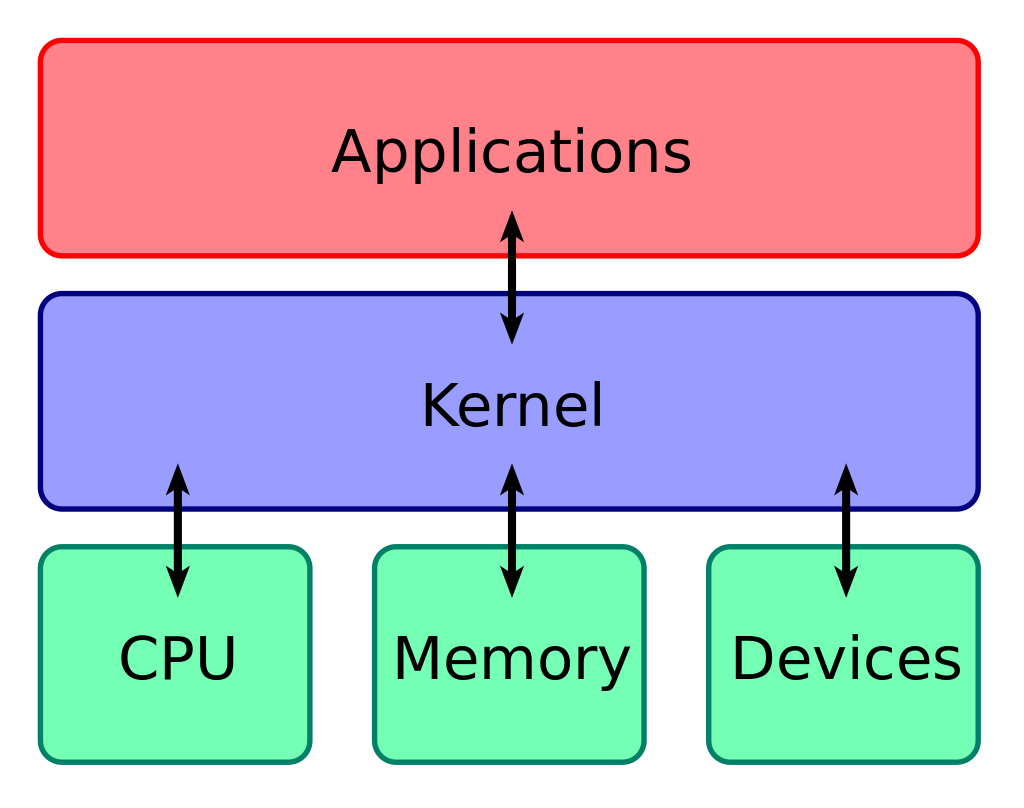
\includegraphics[width=1\columnwidth]{../img/image.png}
		\caption{Example diagram.}
		\label{fig:proposedalgorithm}
	\end{center}
\end{figure} 


\subsection{Limitations and Requirements}
A brief description of the design mechanism's limitations and requirements in accordance with the definitions in Scope and Limitations.


\subsection{Implementation}

A brief description of the implementation and pointer to git where it can be downloaded and tested. \url{https://myalgorithm.com}.

% Results
\chapter{Results}
\epigraph{``A scientist in his laboratory is not a mere technician: he is also a child confronting natural phenomena that impress him as though they were fairy tales.''}{\vspace{10pt}Marie Curie}
\label{chapter:results}
\newpage

This chapter presents the results obtained while evaluating the proposed algorithm/mechanisms. The discussion and analysis of results are presented in the \nameref{chapter:discussion} chapter.


\section{Performance evaluation}
 
\section{Statistical Tool Assumptions Tests}
The evaluation of the assumptions of the statistical tool used should be reported.

\section{Statistical Tool Results}
The results of the statistical tool used are presented in this section.

\section{Obtained Metrics}
Additional metrics obtained during the development of the research are presented in this section. 


\subsection{Most Complex Scenario Metrics (if needed)}


\section{Correctness (if needed)}
If the correctness of the proposal was evaluated, it should be presented in this section.
\section{Output (If needed)}
If the proposal's output differs from what was analyzed with the statistical tool, it should be presented in this section.
\newpage

%Disussion

\chapter{Discussion}
\epigraph{``Another quote.''}{\vspace{10pt}Another Author}
\label{chapter:discussion}

\newpage

This chapter presents the analysis and discussion of the results shown in chapter \nameref{chapter:results}.



%Conclusions and future work
\chapter{Conclusions and Future Work}
\epigraph{``Another quote.''}{\vspace{10pt}Another author}
\label{chapter:conclusions-fw}

\newpage

This chapter presents the final conclusions obtained through the research effort and the future work that can be derived. 

\section{Conclusions}

\begin{itemize}
	
	\item  Conclusion 1.
	
	\item Conclusion 2.
	
	\item Conclusion 3.
	
	
\end{itemize}


\section{Future Work}

\begin{itemize}
	\item Future work 1.
	
	\item Future work 2.
	
	\item Future work 3.
	
\end{itemize}

%Appendix

\chapter{Appendixes}
\label{chapter:appendixes}

\newpage

\section{Source Code}

\label{deliverable:source-code}

%\subsection{General details}
Pointer or description of the source code can be given in this section..

\section{Gathered Data from the Experiments}

If required, raw data could be presented in this section.




% Final pages
\backmatter

% Use single space
\singlespacing

% Bibliography
\cleardoublepage
\renewcommand{\bibname}{References}

\refstepcounter{chapter}
\addcontentsline{toc}{chapter}{\bibname}
\bibliographystyle{plainnat}
\bibliography{mendeley}{}

\doublespacing



\end{document}
